\subsection{三大系统}

\begin{frame}{从 Windows 1.0 到 Windows 11}
    \begin{columns}
        % col 1
        \column{0.3\textwidth}
        \begin{figure}
            \centering
            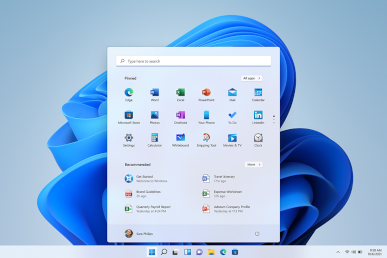
\includegraphics[width=5cm]{Images/windows5.png}
            \caption{Windows 11}
        \end{figure}

        % col 2
        \column{0.6\textwidth}
        \begin{figure}
            \centering
            
\includegraphics[width=0.1\linewidth]{Images/windows3.jpg}
            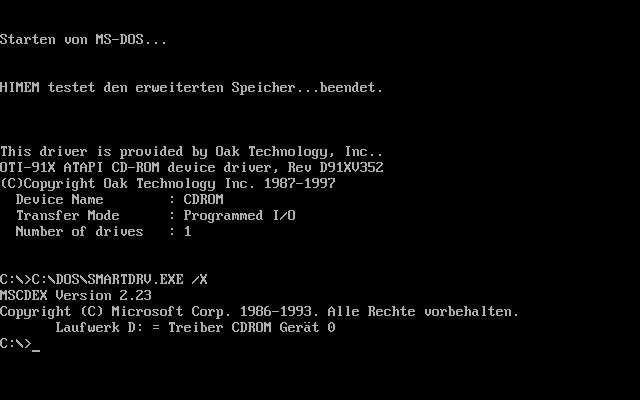
\includegraphics[width=5.2cm]{Images/windows4.png}
            \caption{MS-DOS 命令行界面}
        \end{figure}
        \tiny{现在在 Windows 系统中的 \textcolor{red}{PowerShell} 已经取代了 CMD成为新一代壳程序(Shell), 但是 CMD 仍然集成在操作系统中}
    \end{columns}
    \footnotenoindex{https://zh.wikipedia.org/wiki/Microsoft\_Windows}
    \footnotenoindex{https://zh.wikipedia.org/wiki/File:MS-DOS\_Deutsch.png}
    \footnotenoindex{https://zh.wikipedia.org/wiki/Windows\_11\#/media/File:Windows\_11\_Desktop.png}
\end{frame}

% 接下来, 我们来谈谈操作系统的概念和发展史
% 首先是我们最熟悉的 Windows 操作系统, 左边是现在最新的 Windows 11, 当然现在大部分人应该还在用 Windows 10
% 我们可以用鼠标单机和双击,完成对电脑绝大多数的操作

% Windows1.0 发布于 1985 年, 当年的 Windows 可不是能够用鼠标点点点的, 我们看右边
% 一开始 Windows 系统长这样, 就是一个干巴巴的 DOS 命令行
% 其实现在,这个命令行仍然存在, 也就是大家所知道的 CMD 命令行工具, 它被内置在现代 Windows 系统中
% 当年的电脑,一般人用不了,必须是受过专业训练的程序员才能通过键盘敲入命令的方式控制电脑

% 其实 CMD 它是一种壳程序,英文名叫 Shell 程序,什么是壳程序,或者说 Shell,我们后面会讲
% 那 Windows 发展至今, 其实 CMD 这个 Shell 已经逐渐被 PowerShell 这个功能更强大的 Shell 所取代了
% 不过 CMD 目前和 PowerShell 是在 Windows 中都存在的
% 请大家注意我提到的这个 Shell 概念,我们后面很多的课程都在 Shell 中完成

\begin{frame}{Windows, Linux, MacOS}
    \begin{columns}
        % col 1
        \column{0.5\textwidth}
        \begin{figure}
            \centering
            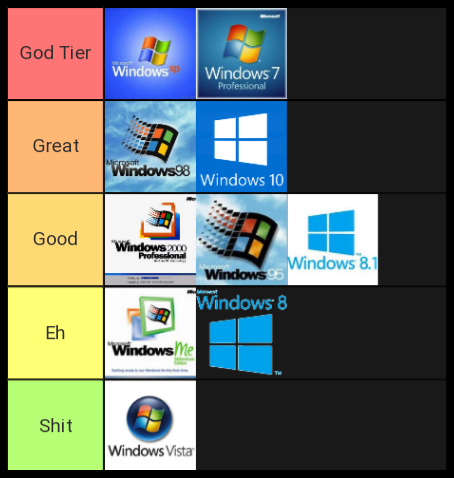
\includegraphics[width=3.5cm]{Images/windows.jpg}
            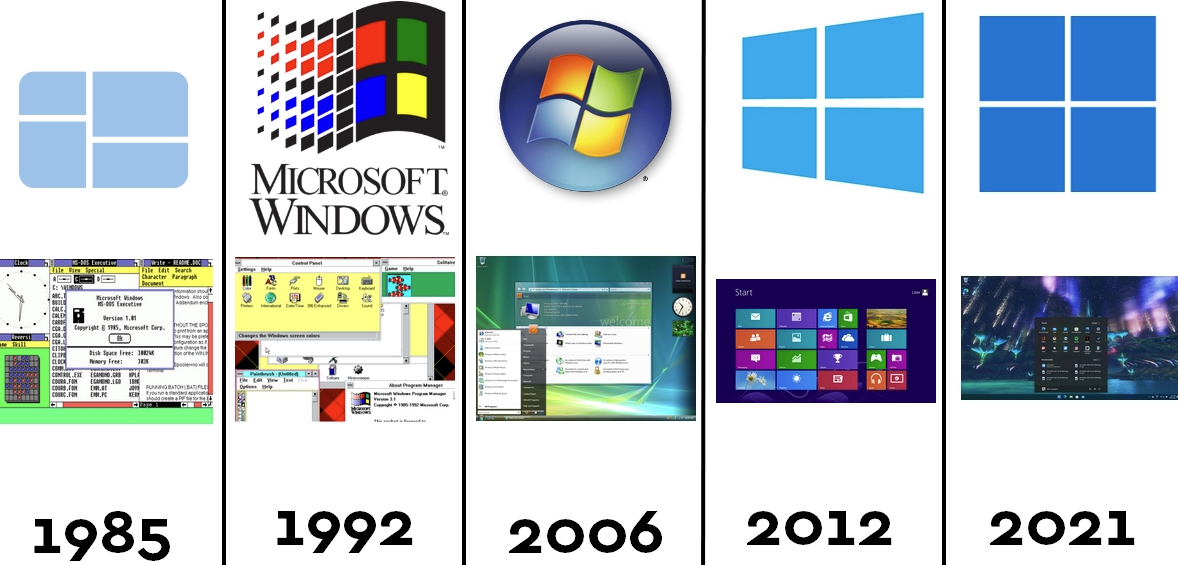
\includegraphics[width=3.5cm]{Images/windows2.jpg}
            \caption{Windows}
        \end{figure}

        % col 2
        \column{0.5\textwidth}
        \begin{figure}
            \centering
            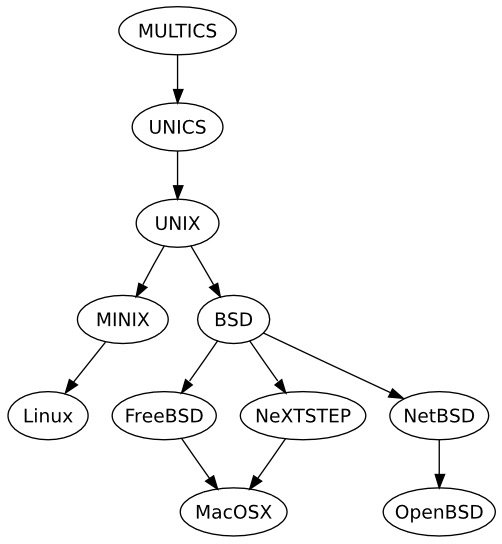
\includegraphics[width=5cm]{Images/unix.jpg}
            \caption{Linux, MacOS起源于UNIX}
        \end{figure}
    \end{columns}
\end{frame}
% 从 1985 年,Windows 系统诞生以后,Windows 就逐渐将系统做成了面向普通大众的,通过可视化的窗口点击来运行的系统,
% 并且每隔几年就推出新的版本,到了现在, Windows 系统已经占据了世界个人电脑操作系统的垄断地位

% 那除了 Windows, 剩下两个系统是什么?
% 在这门课里,三大系统指的分别是 Windows, Linux 和 MacOS

% 而 MacOS 和 Linux 就比较像了,他们都起源于一个叫做 Unix 的操作系统
% 我们刚刚讲到了 Windows 诞生于 1985 年, 而 Unix 系统的诞生时间比 Windows 还要早,
% Unix系统是在 70 年代初期, 在著名的美国贝尔实验室诞生的操作系统
% 贝尔实验室很有名, 它也是 C 语言的发明地,二极管的发明地, 这个实验室的很多研究造就了现在的计算机架构
% 我们说回 Unix
% 而经过几十年的发展, Unix 系统演化为了开源的 Linux 操作系统和专属于苹果公司闭源的 MacOS 操作系统.

\begin{frame}{Windows, Linux, MacOS}
    \begin{columns}
        \column{0.4\textwidth}
        Linux (Open source)

        \begin{itemize}
            \item 上百种不同的发行版\dots
            \item Ubuntu/Debian
            \item CentOS
            \item Android (Google Inc.)
            \item \underline{Shell: (sh, \textcolor{red}{bash}, zsh\dots)}
        \end{itemize}

        MacOS (Apple Inc.)
        \begin{itemize}
            \item Monterey
            \item \underline{Shell: (sh, bash, \textcolor{red}{zsh}\dots)}
        \end{itemize}
        \column{0.6\textwidth}
        \begin{figure}
            \centering
            
\includegraphics[width=6cm]{Images/distros_linux.jpeg}
            \caption{Linux发行版本}
        \end{figure}
    \end{columns}
\end{frame}

% Linux 由于是开源的,谁都能改来用,所以后面发展出了很多发行版本,
% 现在Linux 拥有上百种发行版本
% 比较有名气的比如罗列的 Ubuntu系统和 CentOS 系统
% 其实手机的 Android 操作系统也使用 Linux 的内核, 不过它由谷歌公司掌控, 是半开源状态

% 一般来说 Linux 的壳程序,也就是 Shell 默认是 bash,也可以设置为 sh,zsh 等其他 Shell程序

% MacOS 它是由苹果公司开发和掌控的, 是一个闭源的系统,
% 现在最新版本的系统是 monterey(蒙特雷)
% 而蒙特雷系统中默认的Shell程序 是 zsh,当然也可以设置为 sh 或者 bash

% 请注意我们反复提到了壳程序,或者说 Shell 程序这个概念
% 不断地让这个名字和大家见面,是因为 Shell 这个东西需要大家熟悉,我后面会细讲

% 毕竟 Linux 和 MacOS 是同源的, 可以使用相同的 Shell 程序是非常合理的
% 我们把 Linux比如 Ubuntu CentOS 和 苹果的 MacOS 这种
% 从 Unix 发展而来的操作系统统称为 类 Unix 操作系统

% 现在我们知道了 Windows, 类 Unix 包括 Linux 和 MacOS 
% 都是拥有 Shell 程序的,这是他们的相同点
% 那 Windows 和类 Unix 系统之间的区别是什么呢?

\begin{frame}{Windows与Unix-like系统之间的区别}
    \begin{columns}
        \column{0.5\textwidth}
        \small{
            \begin{table}[h]
                \begin{tabular}{|l|r|r|}
                \hline
                {\textbf{特点}} & {\textbf{Windows}} & {\textbf{Unix-like}} \\ \hline
                参考版本              & Windows10              & Ubuntu20.04              \\ \hline
                是否开源              & 否                      & 是                        \\ \hline
                路径表示              & 反斜杠                    & 斜杠                       \\ \hline
                文件结构              & 分区管理                    & 单一树状                       \\ \hline
                Shell 命令          & CMD 风格                 & Bash 风格                  \\ \hline
                \end{tabular}
        
                \textbf{\normalsize{Windows}}: 
                    \small{\underline{\textcolor{red}{C:}\textbackslash User\textbackslash zhaohuanan\textbackslash Document\textbackslash a.txt}}
                    
                    \small{\underline{\textcolor{red}{D:}\textbackslash somewhere\textbackslash Document\textbackslash b.txt}}

                \textbf{\normalsize{Ubuntu}}: 
                    \small{\underline{\textcolor{red}{/}home/zhaohuanan/Document/a.txt}}

                    \small{\underline{\textcolor{red}{/}home/someone/Document/b.txt}}
            \end{table}
        }
        \column{0.5\textwidth}

        \centering 
        Shell 命令举例

        \tiny{
            \begin{table}[]
                \begin{tabular}{|l|l|l|c|c|}
                \hline
                \textbf{操作}   & \textbf{\begin{tabular}[c]{@{}l@{}}Windows\\ CMD 命令\end{tabular}} & \textbf{\begin{tabular}[c]{@{}l@{}}Ubuntu\\ Bash命令\end{tabular}} & \textbf{相似} & \textbf{不同} \\ \hline
                切换目录          & cd                                                                & cd                                                               & √           &             \\ \hline
                打印当前目录        & cd                                                                & pwd                                                              &             & √           \\ \hline
                清除屏幕          & cls                                                               & clear                                                            &             & √           \\ \hline
                列出文件与子目录      & dir                                                               & \begin{tabular}[c]{@{}l@{}}ls \\ ls -l\end{tabular}              &             & √           \\ \hline
                列出所有文件与子目录    & dir /a                                                            & \begin{tabular}[c]{@{}l@{}}ls -a \\ ls -la\end{tabular}          &             & √           \\ \hline
                创建目录          & \begin{tabular}[c]{@{}l@{}}mkdir\\ md\end{tabular}                & \begin{tabular}[c]{@{}l@{}}mkdir\\ mkdir -p\end{tabular}         & √           &             \\ \hline
                删除目录          & \begin{tabular}[c]{@{}l@{}}rmdir\\ rd\end{tabular}                & \begin{tabular}[c]{@{}l@{}}rmdir\\ rm -rf\end{tabular}           & √           &             \\ \hline
                新建文件          & cd .> | notepad                                                           & touch                                                            &             & √           \\ \hline
                删除文件          & del                                                               & rm                                                               &             & √           \\ \hline
                拷贝文件          & copy                                                      & cp                                                               &             & √           \\ \hline
                在 Shell 中打印文件 & type                                                              & cat                                                              &             & √           \\ \hline
                移动文件          & move                                                              & mv                                                               &             & √           \\ \hline
                展示目录结构        & tree                                                              & tree                                                             & √           &             \\ \hline
                \end{tabular}
            \end{table}
        }
    \end{columns}
\end{frame}
% 首先,他们的区别是 Windows 是商业化的,闭源,微软公司以此盈利, Linux 是开源的,完全免费
% 第二个就是,类 Unix 操作系统和 Windows 的很经典的一个区别,就是文件的路径

% Windows 使用反斜杠来代表文件层级,如 C 盘的 User 目录下的 zhaohuanan 目录下的 Document 下的 a 这个文本文件
% 而windows 的文件系统是分区管理的,也就是说他的根目录出发点可以从 C 盘开始,一层一层往下找,找到 C 盘下的 User 下的 zhaohuanan 下的 Document 下的 a 这个文本文件
% 也可以从 D 盘出发,找打 somewhere 这个目录下的 Document 目录下的 b 这个文本文件
% Windows通过反斜杠来区分文件夹的层级, 而通过赋予这些磁盘 C 盘或者 D 盘或者 EFG 盘这种盘符,来进行分区管理

% 而类 Unix 系统则使用斜杠来代表文件层级, 且以斜杠开头, Unix 所有文件的地址都从这个斜杠开始,
% 而这个斜杠叫根目录
% 所以我们是从根目录出发,来到 home 这个文件夹中,找到 zhaohuanan 这个文件夹,再找到 Document这个文件夹,最终找到了 a 这个文本文件
% 而类 Unix 系统的特点就是你找什么文件和文件夹,都要从根目录出发,比如去找 b 这个文本文件夹,就还是从根目录出发,
% 从 home 到 someone 的 Document 文件夹下找到 b 这个 txt
% 类 Unix 系统是没有分区这个概念的,一切磁盘都从根目录开始寻址

\begin{frame}{文件系统结构}
    \begin{figure}
        \centering
        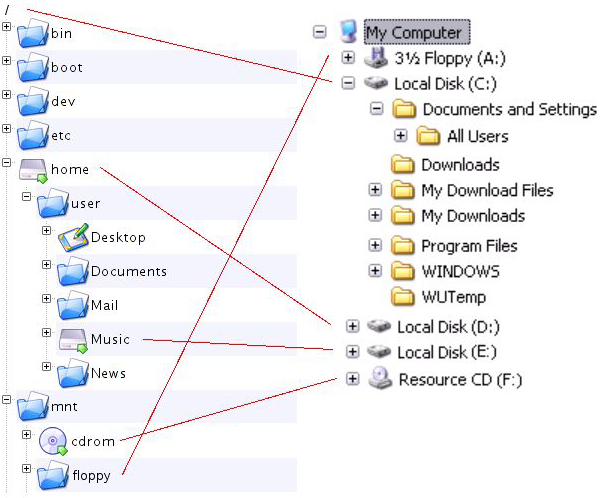
\includegraphics[width=0.55\linewidth]{Images/FileSystemWindowsVsLinux.png}
        % \tiny{\caption{左: 类 Unix 单一树状文件结构; 右: Windows 分区管理文件结构}}
    \end{figure}
    % \footnotenoindex{https://stevevincent.info/LUX205\_2017\_2.htm}
\end{frame}

% 我们用一张图,再来理解一下刚刚讲到的 Windows 和 Linux 文件系统的区别
% 左边是一个 ubuntu系统的文件路径
% 右边是一个windows 系统的文件路径
% 大家可以看到,在 Windows 这个系统中,一些文件路径是并列的,比如我们有一块硬盘分成了 C 盘和 D 盘,我们有另一块硬盘
% 分成一个 E 盘,我们还插入了一个 CD 光盘,系统给它分配了 F 盘, 还插入了一个软盘,给它分配了 A 这个盘符
% Windows 这里的这种文件地址都是以分配一个盘符为开始,然后向下寻址的,比如我要找 CD 光盘中的一个文件,那我要先跳转到 F 盘,再开始寻址

% 而 Linux 在这里就有理念上的不同了, 大家可以看到,我们同样挂载了一个 CD 光盘和一个软盘, 但是 Linux 系统会把他们放在 mnt 这个文件夹里面
% 而原本 Windows 一块硬盘分区为了 C盘 D 盘,在 Linux 就不去做拆分,而原本 Windows 中单独加的一块硬盘 E 盘,就可以
% 挂载到根目录下的 home 目录下的 user 下的 Music 这个路径

% 我们可以感受到 Linux 系统的设计理念,就是把一切都整合到一个树状分支路径中
% 而 windows 的理念就是,你每给我添加一个新的存储设备,我就给你分配一个根目录盘符和一个独立的树状分支

% 那讲到现在,相信大家对 Windows 和 Linux 的文件系统有一定的认识了
% 我们接下来对前面讲到的 Windows 和 Linux 的 Shell 命令以及路径进行一个简单的演示

\begin{frame}[standout]{路径演示}
    \begin{enumerate}
        \item 演示 Windows, MacOS, Linux(以Ubuntu为例)进入文件路径
        \item 打印当前目录, 切换目录
        \item 列出文件与子目录, 列出所有文件与子目录, 创建目录, 删除目录
        \item 新建文件, 拷贝文件, 移动文件, 删除文件
        \item 在 Shell 中打印文件, 清除屏幕
        \item 展示目录结构
    \end{enumerate}
\end{frame}

% -   怎么进入 Windows 的PowerShell
% -   怎么进入 Linux 和 MacOS 的 terminal
% 注意事项:
% 1. 字体调大
% 2. 事先准备好全屏的两个虚拟机可视化窗口
% 3. 争取所有操作全屏下进行

\begin{frame}{演示结论}
    \begin{myoutline}
        \1 类 Unix 系统和 Windows 系统在具体的特点上区别很大
            \2 路径分隔符不同
            \2 文件系统的结构不同
            \2 Shell 命令不同
        \1 但是这些操作系统的抽象层面上的逻辑都是类似的!
            \2 Shell 命令不同, 但具有相同或相似的功能, 如 type 和 cat
            \2 文件系统中的操作具有共性
                \3 文件/文件夹的创建/拷贝/移动/删除
                \3 目录切换
                \3 \dots
    \end{myoutline}
\end{frame}

% 虽然类 Unix 系统和 Windows 系统在具体的特点上区别很大,
% 比如路径分隔符一个用斜杠一个用反斜杠
% 文件系统的结构不同,一个用单一的树状结构,一个用分区结构
% Shell 命令也有很多都不一样

% 但是这些操作系统的抽象层面上的逻辑都是类似的
% 比如,虽然他们 Shell 命令不同, 但具有相同或相似的功能, 如 type 和 cat的功能都是打印文件内容到 Shell 程序中
% 再比如文件/文件夹的创建/拷贝/移动/删除,和目录切换

\begin{frame}{Unix系统层级}
    \begin{columns}
        \column{0.7\textwidth}
        \begin{figure}
            \centering
            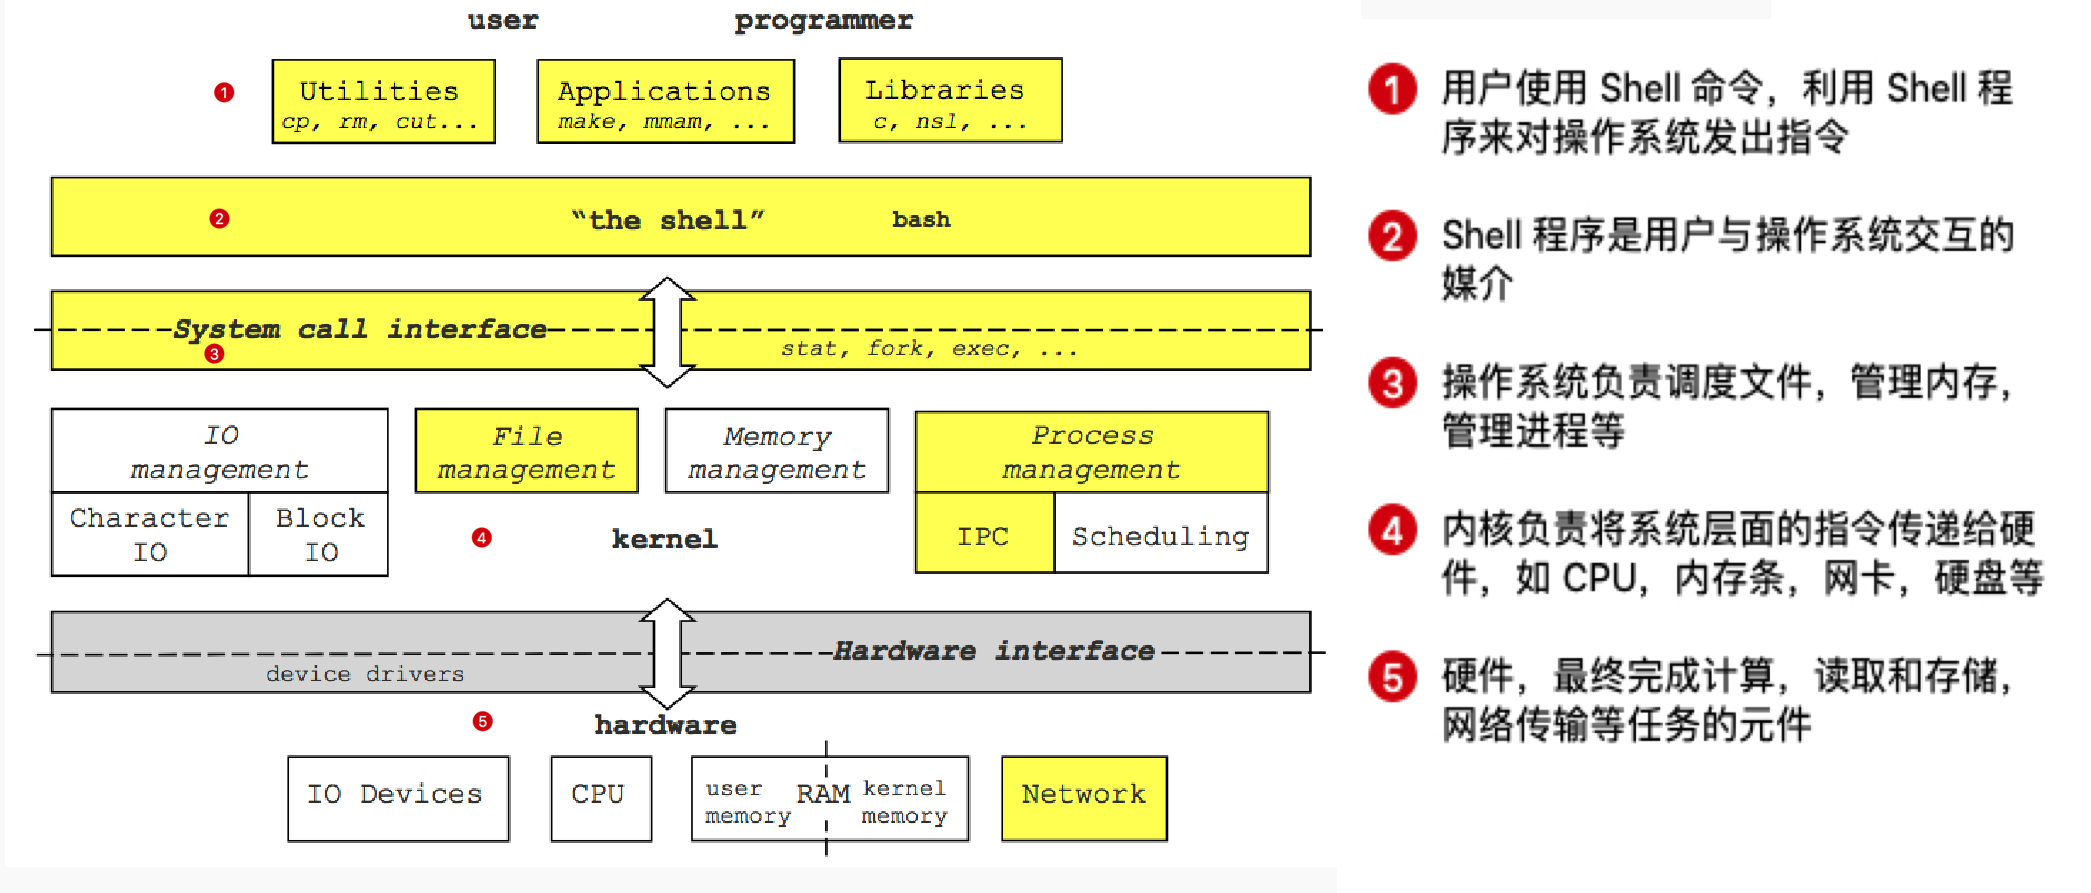
\includegraphics[width=1\textwidth]{Images/linux_work_order.png}
        \end{figure}
        \column{0.3\textwidth}
        \begin{myoutline}
            \1 用户空间
                \2 定义用户可访问的应用程序、库和标准实用程序
                \2 Shell也在``用户空间''中运行
            \1 内核空间
                \2 管理用户操作和硬件之间接口的操作系统的操作
                \2 操作系统的核心部分,其主要工作是将用户应用程序与底层硬件配对,并允许多个程序共享单个硬件组件
            \1 硬件
                \2 计算机的底层物理组件
                \2 输入/​​输出设备,如键盘和显示器、进行计算的 CPU、内存组件和网络接口
        \end{myoutline}
    \end{columns}

    \footnotenoindex{https://classes.adamaviv.com/ic221/s18/units/01/unit.html}
\end{frame}
% 其实 Windows 和 Unix 系统在宏观的逻辑上是非常相似的,
% 我们以 Unix 系统的层级为例来为大家介绍
% 我们使用 Shell 程序中的一个命令,比如说 cp 也就是拷贝文件这个命令,
% 第一步,这个命令会传递给 Shell 程序,
% 第二步,Shell 程序告诉操作系统, 要执行一个文件拷贝操作
% 第三部,这个操作会在操作系统层面发出指令给内核,
% 这个指令的内容包括了,调用一个 IO 指令,把原始文件读入内存, 然后再把内存中的信息写入硬盘
% 第四步,内核将这些指令真正转换为对硬件的一个个操作指令
% 第五步,硬件将这些指令进行执行

% 操作系统就像一个中间的传令兵一样,把我们想做的事情转换为对硬件的指令真正对硬件进行操作

% UNIX的系统层面上把上面这五步可以分为三个主要部分:

% 第一个部分是,用户空间:
% 用户空间定义用户可访问的应用程序、库和标准实用程序。
% Shell 壳程序就是一个用户空间的应用程序
% 我们写程序的时候,就是从用户空间开始操作的,
% 而不必不关心底层硬件之间的差异,那些由开发操作系统和驱动程序的人去关注。
% 那对我们来说, 执行 cp 命令在任何Unix 计算机上都一样,
% 但是由于每台计算机可能硬件不同, 系统底层给硬件的指令可能是不同的

% 第二个部分是内核空间:
% 这是指管理用户操作和硬件之间接口的操作系统的操作。
% 它是操作系统的核心部分,其主要工作是将用户应用程序与底层硬件配对,并允许多个程序共享单个硬件组件。

% 第三个部分是硬件:硬件是计算机的底层物理组件。
% 其中包括输入/​​输出设备,如键盘和显示器、进行计算的 CPU、内存组件和网络接口。

\begin{frame}{Linux的应用场景}
    \begin{myoutline}
        \1 桌面应用
            \2 Ubuntu
            \2 Archlinux
        \1 嵌入式应用
            \2 电梯、汽车、玩具、灯具、冰箱、空调、电饭煲等,都属于嵌入式概念的应用
        \1 服务器应用
            \2 开源, 免费, 无需考虑商业软件授权问题
            \2 高稳定性, 高可靠性
            \2 硬件要求低
    \end{myoutline}
\end{frame}
% 那我们讲了这么多类 Unix 系统的知识,
% 现在,我们来看一下其中的 Linux 系统到底被用来作什么
% 最容易理解的就是个人电脑,也就是桌面应用,这一点 Ubuntu 和 Archlinux等 Linux 系统发行版做得很好很漂亮
% 第二个应用就是嵌入式, 比如我们用的冰箱,洗衣机什么的,对话面板都是属于嵌入式开发,
% 最后,也是 Linux 最为核心的应用,就是用作服务器的系统,

% 讲到这里,我们基本上也进入了本课程的正题了,
% 大家都知道, 生物信息学相关的应用程序大都是基于 Linux 系统的,
% 手机上使用绝大多数需要服务器提供网络服务的 app, 比如 bilibil,知乎, 都是基于 Linux 系统的,
% Linux 系统能相比较于 Windows 和 MacOS,在服务器应用上占据绝大多数市场份额,
% 最大的原因有这三点,
% 首先,相对于 Windows 和 MacOS,Linux 是开源完全免费的
% 其次就是,Linux 系统非常稳定可靠,极少出现类似 Windows 打开一个大型论文文档, 编辑完还没保存就崩溃了这种问题
% 要知道,在大型的商业应用中,服务器如果宕机一个小时,可能对他们来说就会带来几百万的经济损失,
% 在稳定性上 Linux 相比 Windows 和 MacOS 都更值得信赖
% 最后一个点就是,跑起来一个Linux 系统,需要的硬件性能很低,可能一个 256M 的内存就可以跑得动 Linux,当然这是在不装 UI 界面的情况下,
% 而跑起来 Windows 系统起码也要 2G 的内存
% 综合下来, Linux 在服务器上的优势非常明显,所以现在也是占据了绝对主导的地位

% 好,我们花了较长时间来讲解三大系统这一个知识点,是希望大家在后面学习 Python 的过程中能
% 对整个计算机的组成有更深入的理解
% 对文件路径和文件结构有一定的认识
% 那,三大系统这个部分我们就讲完了